\documentclass[11pt,letterpaper]{article}
\usepackage[margin=0.9in]{geometry}
\usepackage{amssymb,amsmath,enumerate,mathtools}
\usepackage{graphics,graphicx}
\usepackage{framed, listings}

\lstset{
    language=C,                            % sets the language for the code
    basicstyle=\scriptsize\ttfamily,       % for the actual code
    morekeywords={printf, time_t, scanf},  % adds keywords
    keywordstyle=\bfseries,                % for keywords
    commentstyle=\scriptsize\ttfamily,     % for comments 
    showstringspaces=false                 % prevents underscores from appearing in output
}

\lstset{
    language=Verilog,                            % sets the language for the code
    basicstyle=\scriptsize\ttfamily,       % for the actual code
    morekeywords={assign, logic, module, endmodule},  % adds keywords
    deletekeywords={if, do, for},               % removes keywords
    keywordstyle=\bfseries\textbf,                % for keywords
    commentstyle=\scriptsize\ttfamily\emph,     % for comments 
    showstringspaces=false                 % prevents underscores from appearing in output
}

\begin{document}
\begin{flushright}
Andrew Scott\\
E155\\
Lab 7\\
November 2, 2015
\end{flushright}

\begin{center}
Lab 7: Advanced Encryption Standard
\end{center}

\noindent\textbf{Introduction}

In this lab, I wrote a AES hardware accelerator. The accelerator reads in a 128 bit plaintext message and a 128 bit key via the SPI protocol and then performs the AES encryption, outputting the 128 bit encrypted message via the SPI protocol.

\noindent\textbf{Design and Testing Methodology}

There was essentially no hardware (breadboard) design to be done this week, since the only breadboard work to be done was connecting Pi pins to FPGA pins.

For the software (Verilog), I decided to use the datapath/controller design to create a circuit that would execute one round of the encryption algorithm each clock cycle. I achieved this by having a 3mux leading into a register which then fed into a module that performed the AddRoundKey part of the encryption. The 3mux chooses between the first plaintext input, the output from a module performing the MixColumns part of the encryption, and the output from the ShiftRows module part of the encryption (depending on the current round of encryption being performed). The signal controlling the 3mux comes from my controller module which has a finite state machine inside it that keeps track of the current round. The implementations of AddRoundKey and ShiftRows were simple, and the implementations for MixColumns and SubBytes were given (SubBytes just required writing a wrapper function to call the given SubByte module on each of the individual bytes in the plaintext). The AddRoundKey implementation was simple because it is just an XOR with a round key, but generating the round key itself turned out to be quite a bit of work. My key expansion module to generate this round key ended up resembling a datapath on its own, generating the 128 bit key each round (representing 4 executions of the key expansion loop in Figure 11 of the AES standard). This datapath has a 2mux control signal coming from the aes controller module. The point of this 2mux is to choose between the original input key on the first round and the key generated on the previous round for the rest of the rounds. I put a register to hold the current key which has as input the output from the 2mux described before. The first 32 bits of the new key go through a module that performs the \verb|temp = SubWord(RotWord(temp)) xor Rcon[i/Nk]| line from the key expansion pseudocode. I then had a series of XOR gates performing the \verb|w[i] = w[i-Nk] xor temp| line for each of the 32 bit segments of the new key. The resulting new key was then stored in the key register and then used to generate the next key on the next clock cycle. I tested my implementation using the provided testbench, which helped me to find several bugs (one of which was the fact that I wasn't maintaining the value of the encrypted message after encrypting it, which was solved by simply making my registers write-enabled).





\noindent\textbf{Results and Discussion}\\
I was able to complete the entire lab, and as far as I can tell everything is working properly. Running the provided C code on the Pi sends over a plaintext message and a key and the received encrypted message is correct. This works for both of the provided test cases.

\noindent\textbf{Conclusion}\\
I unfortunately spent more than an hour trying to debug my physical hardware on the breadboard and the pin assignments from the Quartus pin planner since I was working on the lab before the problem with the EasyPIO.h file came to light, but fortunately I was eventually able to get everything working. In total I spent about 10 hours on this lab.


\pagebreak

\noindent\textbf{Breadboard Schematic}\\\\
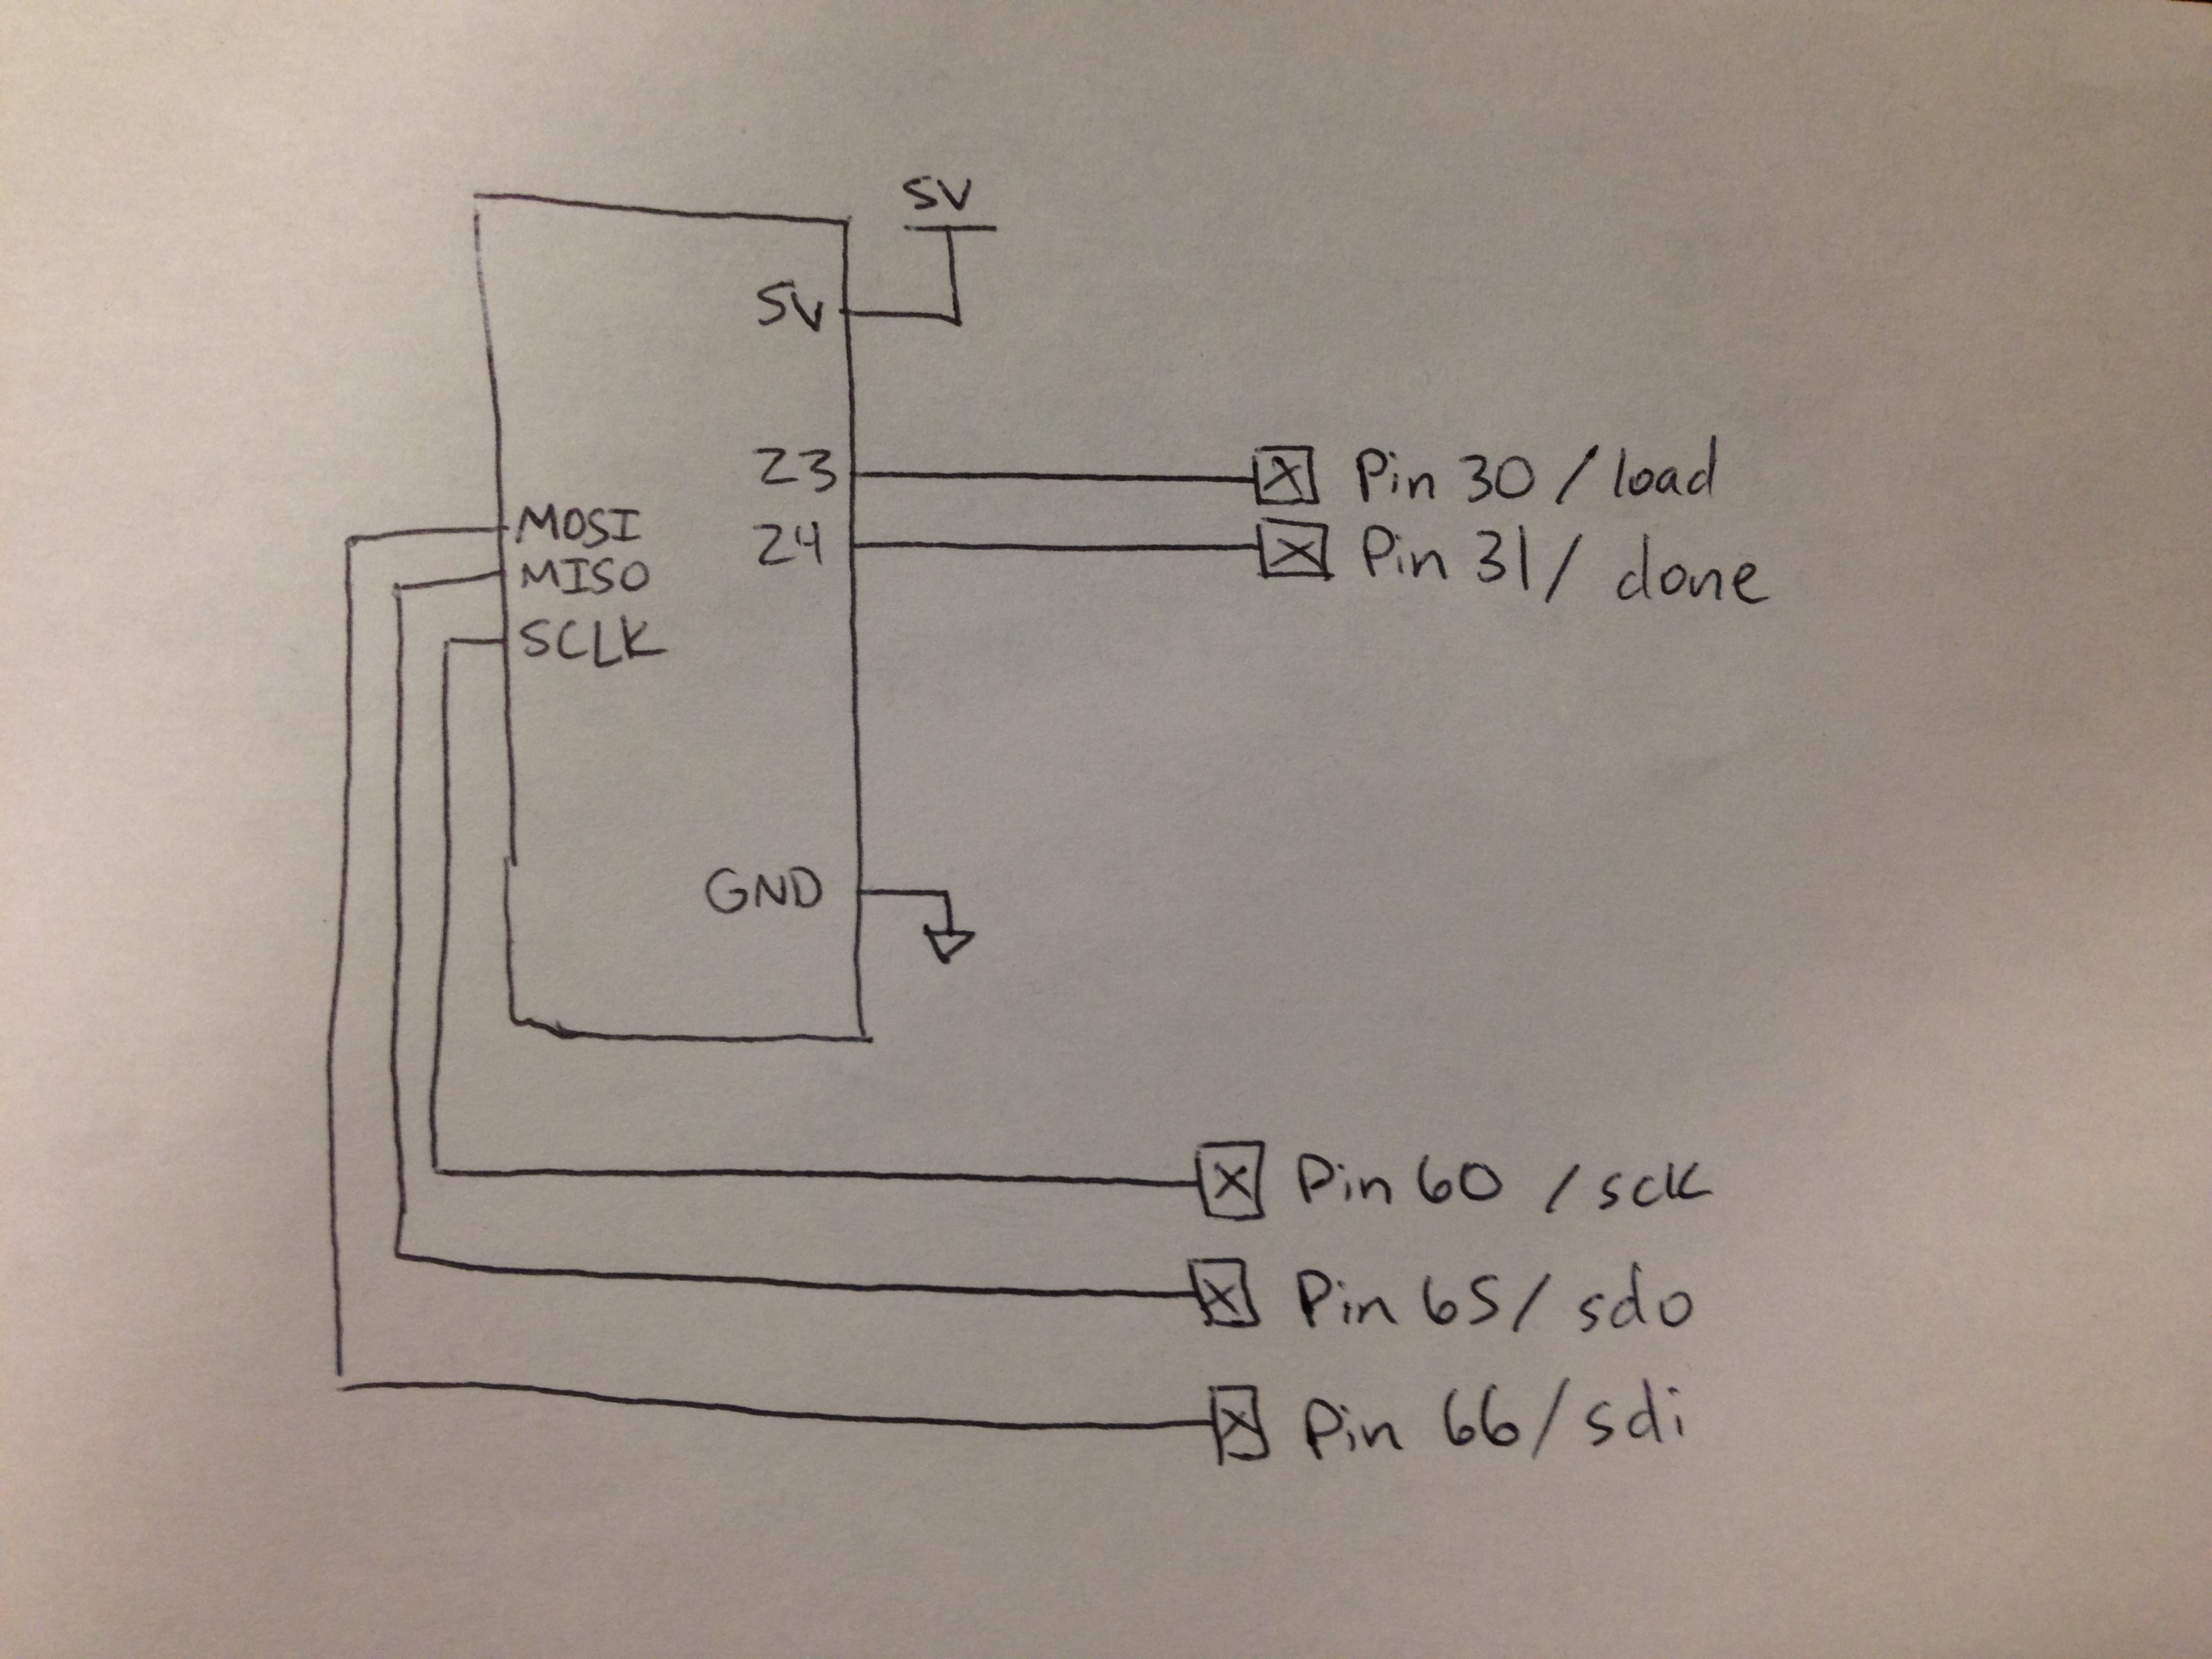
\includegraphics[scale=0.15]{lab7schematic}


\noindent\textbf{Verilog}\\
\lstset{language=Verilog}
\noindent\textbf{aes.sv}
\lstinputlisting{aes.sv}

\noindent\textbf{C Code}\\
\lstset{language=C}
\noindent\textbf{lab7.c}
\lstinputlisting{lab7.c}

\end{document}

